%% DONE
\id{IRSTI 28.23.29}{https://doi.org/10.58805/kazutb.v.1.26-728}

\begin{articleheader}
\sectionwithauthors{A. Bolatova, U. Kylyshbek, A. Baktygaliyev, A. Kartbayev}{OPTIMIZING PROJECT DEVELOPMENT RISKS AND MARKET VOLATILITY USING DEEP LEARNING METHODS}

{\bfseries
A. Bolatova\alink{https://orcid.org/0009-0007-8674-7306},
U. Kylyshbek\alink{https://orcid.org/0009-0008-1386-2984},
A. Baktygaliyev\alink{https://orcid.org/0000-0001-6163-4451},
A. Kartbayev\textsuperscript{\envelope } \alink{https://orcid.org/0000-0003-0592-5865}}
\end{articleheader}

\begin{affiliation}
\emph{Kazakh-British Technical University, Almaty, Kazakhstan}

\raggedright \textsuperscript{\envelope }{\em Correspondent-author: a.kartbaev@kbtu.kz}
\end{affiliation}

This study addresses computer modeling challenges by focusing on the
risks in IT projects, with particular emphasis on managing investment
processes under conditions of uncertainty and incomplete information.
The growing number of IT projects in recent years has brought new
challenges to assessing and managing associated risks. As technology
advances and IT initiatives expand in scale, uncertainties in investment
processes have intensified, requiring more sophisticated evaluation
methods. The study introduces a RIC methodology for calculating the risk
function of investment projects, incorporating fluctuations in projected
cash flows. Investment project development is often characterized by
uncertainty and a lack of robust statistical data, necessitating
advanced analytical approaches for sound decision-making. This research
applies modern scientific techniques, including machine learning and
convolutional neural networks, to develop an algorithm for risk
assessment in investment projects. The proposed algorithm provides
practical recommendations to improve the evaluation and management of
investment-related risks. The findings of this study offer valuable
tools for planning and risk analysis, making them applicable to various
stakeholders engaged in investment activities.

{\bfseries Keywords:} investment risk, IT projects, fuzzy fields,
information uncertainty, Big Data, CNN models, machine learning.

\begin{articleheader}
{\bfseries ТЕРЕҢ ОҚЫТУ ӘДІСТЕРІН ПАЙДАЛАНУ АРҚЫЛЫ ЖОБАЛАРДЫ ДАМЫТУ ТӘУЕКЕЛДЕРІН ЖӘНЕ НАРЫҚТЫҢ ҚҰБЫЛМАЛЫЛЫҒЫН ОҢТАЙЛАНДЫРУ}

{\bfseries
А. Болатова,
У. Кылышбек,
А. Бақтығалиев,
А.Картбаев\textsuperscript{\envelope }}
\end{articleheader}

\begin{affiliation}
\emph{Қазақстан-Британ техникалық университеті, Алматы, Қазақстан,}

\emph{e-mail: a.kartbaev@kbtu.kz}
\end{affiliation}

Бұл зерттеу компьютерлік модельдеу мәселелерін шешуге арналған, әсіресе
ақпараттық технологиялар (АТ) жобаларындағы тәуекелдерге, сондай-ақ
белгісіздік және толық емес ақпарат жағдайында инвестициялық процестерді
басқаруға ерекше назар аударады. Соңғы жылдары АТ жобаларының санының
өсуі тәуекелдерді бағалау және басқару бойынша жаңа қиындықтарды
тудырды. Технологиялар дамып, АТ бастамаларының ауқымы кеңейген сайын,
инвестициялық процестердегі белгісіздіктер күшейіп, неғұрлым күрделі
бағалау әдістерін қажет етеді. Зерттеуде инвестициялық жобалардың
тәуекел функциясын есептеуге арналған RIC әдістемесі ұсынылған, ол
болжанған ақша ағындарының ауытқуларын ескереді. Инвестициялық жобаларды
әзірлеу жиі белгісіздікпен және сенімді статистикалық деректердің
жетіспеушілігімен сипатталады, бұл негізделген шешімдер қабылдау үшін
заманауи аналитикалық тәсілдерді қолдануды талап етеді. Бұл зерттеуде
инвестициялық жобалардың тәуекелдерін бағалау алгоритмін әзірлеу үшін
машиналық оқыту және конволюциялық нейрондық желілер сияқты заманауи
ғылыми әдістер қолданылады. Ұсынылған алгоритм инвестициялық
тәуекелдерді бағалау және басқаруды жақсарту бойынша практикалық
ұсыныстар береді. Зерттеу нәтижелері жоспарлау және тәуекелдерді талдау
үшін құнды құралдарды ұсынады және инвестициялық қызметке қатысатын
түрлі мүдделі тараптарға қолданыла алады.

{\bfseries Tүйін сөздер:} инвестициялық тәуекел, АТ жобалары, анық емес
өрістер, ақпараттық белгісіздік, үлкен деректер, CNN үлгілері, машиналық
оқыту.

\begin{articleheader}
{\bfseries ОПТИМИЗАЦИЯ РИСКОВ РАЗРАБОТКИ ПРОЕКТА И ВОЛАТИЛЬНОСТИ РЫНКА С ИСПОЛЬЗОВАНИЕМ МЕТОДОВ ГЛУБОКОГО ОБУЧЕНИЯ}

{\bfseries
А. Болатова,
У. Кылышбек,
А. Бактыгалиев,
А.Картбаев\textsuperscript{\envelope }}
\end{articleheader}

\begin{affiliation}
\emph{Казахстанско-Британский технический университет, Алматы,
Казахстан,}

\emph{e-mail: a.kartbaev@kbtu.kz}
\end{affiliation}

Данное исследование посвящено решению задач компьютерного моделирования,
сосредотачивая внимание на рисках в ИТ-проектах, с особым акцентом на
управление инвестиционными процессами в условиях неопределенности и
неполной информации. Рост числа ИТ-проектов в последние годы привел к
появлению новых вызовов, связанных с оценкой и управлением
сопутствующими рисками. По мере развития технологий и расширения
масштабов ИТ-инициатив неопределенность в инвестиционных процессах
усиливается, требуя более сложных методов оценки. В исследовании
предлагается методология RIC для расчета функции риска инвестиционных
проектов с учетом колебаний прогнозируемых денежных потоков. Разработка
инвестиционных проектов часто характеризуется неопределенностью и
недостатком надежных статистических данных, что требует применения
современных аналитических подходов для принятия обоснованных решений. В
данном исследовании применяются современные научные методы, включая
машинное обучение и сверточные нейронные сети, для разработки алгоритма
оценки рисков в инвестиционных проектах. Предлагаемый алгоритм содержит
практические рекомендации по улучшению оценки и управления
инвестиционными рисками. Результаты исследования предлагают ценные
инструменты для планирования и анализа рисков, которые могут быть
применимы различными заинтересованными сторонами, участвующими в
инвестиционной деятельности.

{\bfseries Ключевые слова:} инвестиционный риск, ИТ-проекты, нечеткая
логика, неопределенность, Большие данные, модели CNN, машинное обучение.

\begin{multicols}{2}
{\bfseries Introduction.} In recent years, the increasing number and
complexity of Information Technology (IT) projects have posed
significant challenges in assessing and managing associated risks. The
rapid advancements in technology and the growing scale of IT initiatives
have amplified uncertainties, particularly in investment processes,
requiring more sophisticated and reliable evaluation methods. In
today' s dynamic business environment, IT infrastructure
and architecture are critical investments that command significant
financial resources. These investments are crucial for constructing
advanced production environments and operational IT architectures. The
investments cover a wide spectrum, including projects, computers,
telecommunications, and services. These are integral to enhancing a
company' s productivity and operational efficiency. Yet,
assessing the return on these investments poses a challenge, often
taking years to realize their full benefits.

Recent scholarly and professional investigations have focused on
evaluating the impact of IT investments on business performance. Various
approaches have been suggested to assess these investments effectively
and efficiently. \emph{McKinsey} reports that IT infrastructure has
undergone significant evolution-from small setups with few servers to
massive data centers with thousands of servers. This transformation is
driven by the need for robust systems capable of supporting essential
business functions like transaction processing, customer data
management, and complex decision-making processes. Investing in IT
infrastructure brings substantial benefits. Well-integrated IT systems
can improve real-time data collection, support extensive analytics, and
enhance market responsiveness, thereby providing a competitive edge. For
example, sophisticated infrastructure allows quicker establishment of
sales offices in emerging markets and improved customer support.

Despite these benefits, the high costs and long commitments required for
developing IT infrastructure present considerable challenges. The
complexity of managing and integrating diverse technologies demands
careful planning and strategic investments. Beyond individual companies,
the strategic importance of infrastructure investments impacts broader
economic activities. Enhancements in digital connectivity and transport
networks facilitate business operations and can significantly boost
economic growth by reducing costs, improving mobility, and bolstering
competitiveness.

From the perspective of Ilin et al., the development and implementation
of Enterprise Architecture (EA), including its IT components,
significantly enhance transparency in business operations and agility in
business re-engineering. They advocate for investment and assessment
models that provide numerous advantages, such as enabling integrated
comparisons of the impact of adopting IT solutions versus fragmented
deployment, more precise calculations of investment project costs,
reduced investment cycles for both physical and IT components, and the
application of international software standards like COSMIC-ISO 19761
for practical implementation {[}1{]}. As well, a research by Purwita and
Subriadi shows how IT investment valuations are influenced by both
tangible and intangible benefits {[}2{]}.

In another study, researchers analyzed Health Information Technology
(HIT) investments in relation to hospital financial outcomes using
econometric and microeconomic techniques. They optimized investment
distribution based on productivity associated with each input,
determining the appropriate investment levels for a global portfolio to
achieve a desired confidence level {[}3{]}. Ali et al. underscores the
significance of Information Technology Investment Governance (ITIG) as a
vital organizational competency, highlighting its role in enhancing the
relationship between IT investments and business performance, based on
resource-based theory {[}4{]}. Berghout' s research
emphasizes the benefits of developing detailed business cases for IT
projects, arguing that while resource-intensive, these cases are
critical for organizations engaging in unfamiliar IT projects by
providing a deeper understanding of the project' s
business value and supporting informed decision-making {[}5{]}.

Further, Chen et al. proposes the development of an effective IT
investment decision model for global organizations, aiming to
demonstrate the framework' s utility in supporting IT
investment decisions {[}6{]}. Additionally, Witra et al. study on gender
and IT investment decision-making reveals that women's risk-averse
behavior has significant implications for investment efficiency,
especially in complex calculations {[}7{]}. Mirza et al. research
suggests that female managers enhance asset efficiency and help
organizations reduce unnecessary expenditures, particularly in
developing economies {[}8{]}. Shin's research further supports the idea
that female directors strengthen board monitoring, impacting
decision-making processes significantly {[}9{]}. Lee' s
research focuses on the critical need for businesses to understand how
technology investments contribute to business outcomes, rather than just
the technological aspects themselves. The study links IT spending to
business growth and stresses the importance of prioritizing investments
that produce tangible bottom-line results, navigating the so-called IT
paradox effectively {[}10{]}.

{\bfseries Materials and Methods.} This research aims to establish a robust
quantitative model to evaluate the effectiveness of IT investments in
promoting business growth, using real-world data. The core proposition
is that by strategically focusing IT investments on areas that generate
substantial bottom-line results, businesses can optimize their expansion
and performance. To achieve this, the study introduces a novel
evaluation method named "RIC" which incorporates three critical
criteria:

1. {\bfseries Risk Score:} This metric assesses the attractiveness of an
investment based on its risk level. The score ranges from 0\%
(indicating very high risk) to 100\% (indicating very low risk),
providing a straightforward, quantifiable measure to gauge potential
risk associated with each IT investment.

2. {\bfseries Return on Investment (ROI):} ROI is used to measure the
profitability of an investment by comparing the return or profit
generated against the initial investment cost. This criterion is
essential for assessing the potential financial gains or losses from
IT investments and supports decision-making by highlighting the
efficiency and effectiveness of the expenditure.

3. {\bfseries Criteria yet unspecified:} The third criterion, which will be
detailed further in the study, complements the Risk Score and ROI to
provide a comprehensive view of the investment's value.

The RIC method' s integration of these criteria aims to
provide a multidimensional analysis of IT investments, enabling
organizations to make informed, data-driven decisions that align IT
spending with strategic business objectives. This approach not only
seeks to clarify the direct impact of IT investments but also to guide
companies in prioritizing investments that promise the most significant
returns, thereby enhancing their competitive edge and operational
efficiency.

This research commenced with the use of Python libraries to
systematically gather and process investment-related datasets from a
variety of sources, aiming to build a comprehensive foundation for the
analysis. The primary dataset utilized was the "Twitter Dataset"
obtained from \emph{Kaggle}, which encompasses approximately 1.5 million
tweets and 1.2 GB. These tweets were analyzed to extract insights
related to financial markets and investment trends.

Additionally, it's been integrated a substantial dataset provided by
\emph{McKinsey}, which includes detailed records of around 500 million
interactions from regular users engaging with retail services. This
dataset was pivotal in understanding consumer behavior and its impact on
retail investment trends. The data collection also extended to financial
markets, specifically through the use of data from \emph{Yahoo Finance}.
This source provided daily updates on a selected range of US-listed
financial instruments. Although this dataset is comprehensive, it is
important to note that it may contain some gaps, possibly due to the
selective criteria used in data compilation, which could influence the
availability of complete historical data.

To ensure a robust analytical framework, these datasets were
meticulously cleaned and pre-processed to address inconsistencies and
prepare them for integrated analysis. The aim was to correlate the risks
derived from social media and consumer behavior with actual market
movements, thereby providing a multi-dimensional perspective on
investment strategies and market dynamics. This approach allowed us to
harness big data analytics to derive actionable insights that could
potentially guide investment decisions and strategy formulation.
\end{multicols}

\begin{figure}[H]
	\centering
	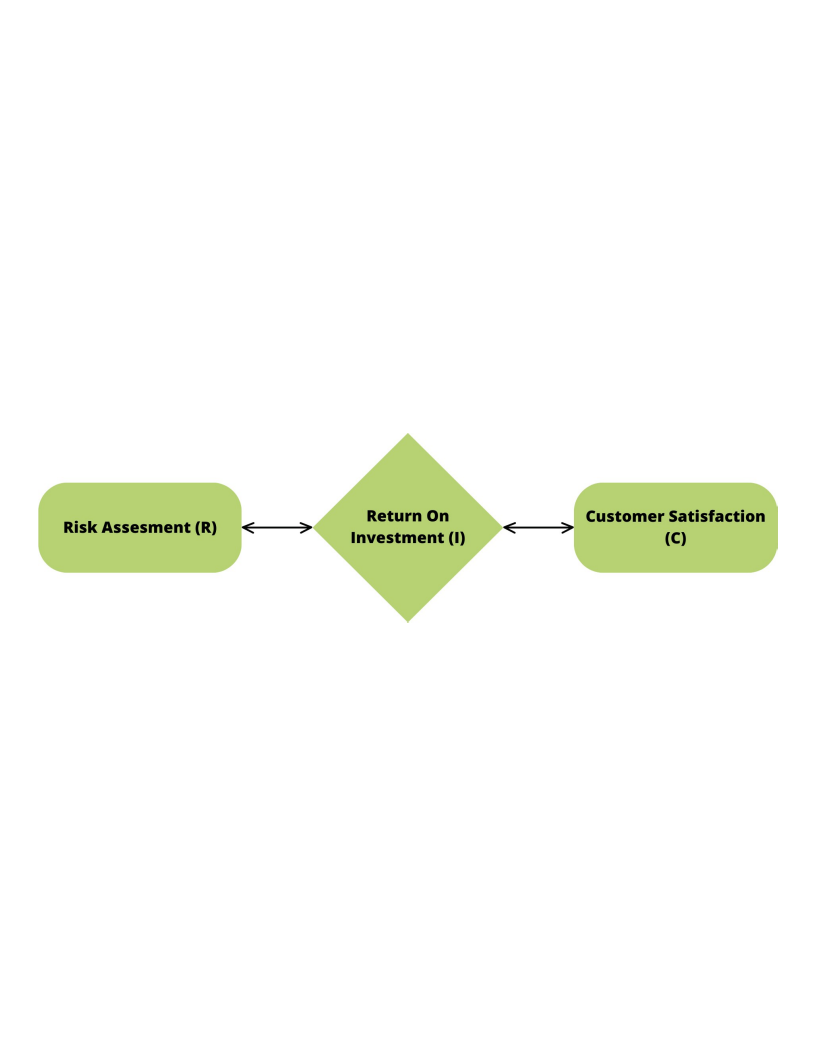
\includegraphics[width=0.6\textwidth]{media/ict2/image9}
	\caption*{Fig. 1 - RIC methodology}
\end{figure}

\begin{multicols}{2}
It has been considered quantitative methods as a cornerstone of the
research, as a way to explore something better. In order to solve the
investment problem, it has been created a method called RIC and uses
three criteria (See Fig.1).

1. R stands for Risk (Risk Assessment)

2. I stands for Investment (Return On Investment)

3. C stands for Customer (Customer Satisfaction)

\begin{equation}
RIC = \frac{R + I + C}{3}
\end{equation}

Each criterion is responsible for the main investment parameters: 1)
both tangible and intangible; 2) tangible; 3) intangible, so that the
method produces the best predictable result. In the realm of investment,
accurately gauging the risk associated with stocks is paramount for
determining their attractiveness and potential returns. The "Risk Score"
is a fundamental metric developed to quantify this aspect, ranging from
0\% to 100\%. A score of 0\% indicates a very high risk, suggesting that
the investment is highly volatile or uncertain. Conversely, a score of
100\% represents a very low risk, pointing to a stable and secure
investment.

Investors rely on the Risk Score to make informed decisions by
evaluating various factors that contribute to the risk profile of an
investment. These factors include market volatility, which reflects the
frequency and magnitude of price fluctuations; economic conditions, such
as inflation rates, employment levels, and GDP growth, which can affect
the overall investment climate; regulatory risks, involving changes in
laws and regulations that could impact business operations;
technological risks, particularly relevant in sectors where rapid
innovation can render existing technologies obsolete; and operational
risks, which encompass issues related to internal processes, systems,
and people.

Understanding these risks is crucial as they directly influence the
potential returns from an investment. By integrating the Risk Score into
their analysis, investors can align their investment choices with their
risk tolerance and investment objectives, aiming to optimize their
portfolios for both risk and return. This approach to risk assessment
not only aids in identifying potentially lucrative investments but also
helps in mitigating potential losses, making it an indispensable tool in
the financial decision-making process. ROI measures the profitability of
an investment by comparing the return or profit generated to the initial
investment cost. It helps assess the potential financial gains or losses
associated with an investment.

\begin{equation}
ROI = \frac{Profit}{CostofInvestment} \times 100
\end{equation}

Measuring customer satisfaction is a critical aspect of evaluating
business performance and understanding the effectiveness of various
investments. One common method to gauge this is through customer surveys
or feedback mechanisms, which can collect detailed insights from
customers about their experiences and satisfaction levels. These results
are often quantified and reported as a percentage of satisfied
customers. This percentage provides a direct indicator of how well a
company is meeting customer expectations and needs. It is a valuable
metric because it offers a clear, numerical benchmark that businesses
can track over time and use to implement improvements. For instance, a
high percentage of satisfied customers generally correlates with better
customer loyalty, repeat business, and positive word-of-mouth, all of
which are crucial for long-term success.

Businesses might utilize various tools for this purpose, including
electronic surveys, feedback forms, social media interactions, and
review platforms. By analyzing the data collected from these sources,
companies can identify strengths and weaknesses in their products or
services and make informed decisions to enhance customer satisfaction.
This process not only helps in retaining existing customers but also
attracts new ones by showcasing the company's commitment to meeting
their needs and expectations.

Further it's been possible to conceptualize a model where the change in
customer satisfaction over time is a function of various factors. Let
\(S(t)\) represent the customer satisfaction level at time \(t\),
measured as the percentage of satisfied customers. To model the change
in satisfaction over time as a function of factors such as improvements
in service quality \((Q(t))\), responsiveness to feedback \((R(t))\),
and changes in customer expectations \((E(t))\) was developed an
equation that can be:

\begin{equation}
\frac{dS}{dt} = k_{1} \cdot \frac{dQ}{dt} + k_{2} \cdot \frac{dR}{dt} - k_{3} \cdot \frac{dE}{dt},
\end{equation}

where:

- \(\frac{dS}{dt}\) is the rate of change of customer satisfaction.

- \(\frac{dQ}{dt},\frac{dR}{dt}\), and \(\frac{dE}{dt}\) represent the
rates of change in service quality, responsiveness, and customer
expectations, respectively.

- \(k_{1},k_{2}\), and \(k_{3}\) are constants that determine the
sensitivity of customer satisfaction to changes in each of these
areas.

This model assumes that improvements in service quality and
responsiveness directly contribute to increasing satisfaction, whereas
rising customer expectations might decrease it. The constants \(k_{1}\),
\(k_{2}\), and \(k_{3}\) would need to be empirically determined based
on data specific to a company or industry.

One of the RIC framework' s key advantages is its
adaptability to integrate advanced machine learning models, such as
convolutional neural networks (CNNs). While it's traditionally
associated with image recognition, their utility in analyzing financial
data lies in their ability to process sequential and structured datasets
with remarkable precision. CNNs can be adapted to handle financial
time-series data by treating the temporal progression of market events
as layers of interconnected features. This approach enables the
extraction of patterns and trends that might otherwise remain obscured.
For example, in the context of the RIC framework, it could analyze
multi-dimensional data inputs such as historical price movements,
trading volume, sentiment scores, and macroeconomic indicators. The
architecture's convolutional layers can identify relationships between
these variables, while pooling layers reduce dimensionality, ensuring
efficient computation. Dilated convolutions could further expand the
receptive field, capturing broader market contexts without increasing
computational overhead. See in Fig.2 more details of the model used for
risk analysis.
\end{multicols}

\begin{figure}[H]
	\centering
	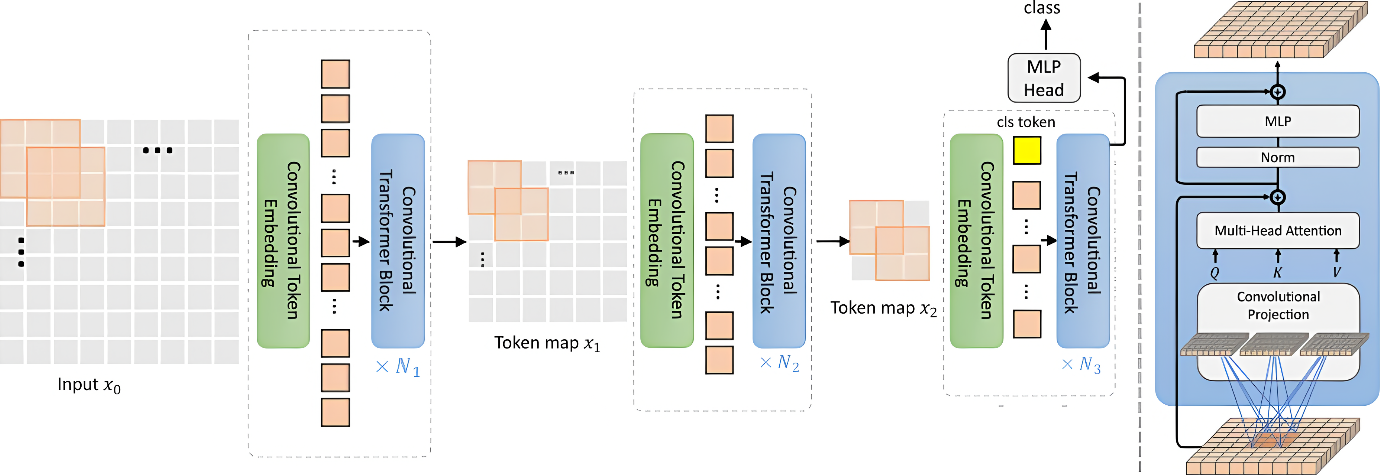
\includegraphics[width=0.8\textwidth]{media/ict2/image10}
	\caption*{Fig. 2 - Design of the CNN model for this study}
\end{figure}

\begin{multicols}{2}
The CNN architecture was originally designed to address image generation
problems. A key component of CNNs is the use of convolutions, which play
a central role in feature extraction. Causal convolutions, in
particular, are employed to preserve the temporal ordering of data,
ensuring that the model's output at timestep \emph{t} depends only on
current and past timesteps, and not on any future information.
Additionally, the architecture incorporates dilated convolutions, which
skip input values at regular intervals. This design enables the
receptive field to expand exponentially with depth, effectively
capturing broader context in the data. CNNs have demonstrated remarkable
success in tasks such as music audio modeling and speech recognition.
Specifically, the dilated causal convolution layers in the architecture
are instrumental in capturing long-term dependencies, making them
well-suited for sequential data modeling.

Due to the nature of the model, which greedily selects the highest and
lowest risk points within a range, a few challenges arise in identifying
risks. Firstly, selecting CNN parameters involves balancing complexity
and efficiency. Typical architectures use 3--5 convolutional layers with
3×33 times 33×3 or 5×55 times 55×5 kernels, a stride of 1 or 2, and ReLU
activation Pooling layers, typically max pooling with a 2×22 times 22×2
window, are used to reduce spatial dimensions while retaining important
features. The number of filters often increases in deeper layers,
starting from 32 or 64 in initial layers and scaling up to 256 or 512 in
later layers to capture complex patterns. Learning rates between 0.001
and 0.0001, tuned via optimizers like Adam or SGD with momentum, ensure
stable and effective training. These parameter choices help build a CNN
that generalizes well across different datasets, as shown in Table 1.

Specifically, the sizes of buying points (peaks) and selling points
(valleys) are relatively smaller compared to holding points. In the
dataset, buying and selling risks account for only 3\% of the total
data, highlighting a significant class imbalance. To address this
imbalance, it's been proposed a sampling method that adjusts the data
distribution based on the rate of rare events, ensuring a more balanced
representation for effective model training, as shown in Fig.3.
\end{multicols}

\begin{figure}[H]
	\centering
	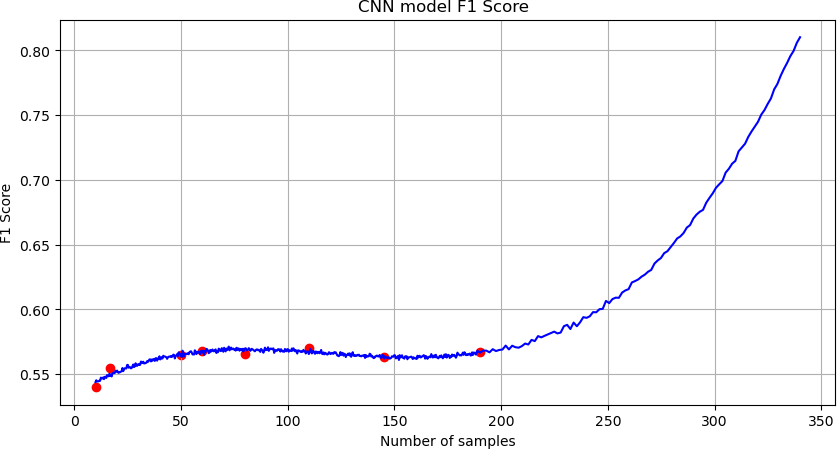
\includegraphics[width=0.8\textwidth]{media/ict2/image11}
	\caption*{Fig. 3 - Evaluation of the CNN model after sampling}
\end{figure}

\begin{table}[H]
\caption*{Table 1 - Comparison of CNN and machine learning models over 350 samples}
\centering
\begin{tblr}{
  cells = {c},
  hlines,
  vlines,
}
Model                          & Accuracy & Precision & Recall & F1-Score \\
Proposed CNN Model             & 92.5     & 93.1      & 91.8   & 92.4     \\
The Hybrid Model [14]          & 88.3     & 87.9      & 88.0   & 87.9     \\
Random Forest [16]             & 85.7     & 84.5      & 86.2   & 85.3     \\
Regression model [15]          & 84.2     & 83.0      & 85.0   & 84.0     \\
Autoregressive (AR)~model [19] & 89.1     & 88.7      & 89.5   & 89.1     
\end{tblr}
\end{table}

\begin{multicols}{2}
In the Table 1, the study highlights the superior performance of the
proposed CNN model, which outperforms traditional machine learning
models and a previous hybrid model in terms of accuracy, precision,
recall, and F1-score. The improvement in performance demonstrates the
effectiveness of the updated CNN architecture, likely due to better
hyper parameter tuning, deeper layers, and optimized feature extraction
techniques.

{\bfseries Results and discussion.} To validate the effectiveness of the
Risk, Investment, and Compliance (RIC) method in assessing investment
opportunities, the study utilized historical data from several
authoritative financial analytics sources. Specifically, data spanning
the past five years from Macrotrends {[}11{]}, Infront Analytics
{[}12{]} and Comparably {[}13{]} were employed to analyze the investment
potential of ten selected companies across various industries.

This approach involved a systematic evaluation of each
company' s performance and market behavior using the RIC.
This formula integrates multiple financial indicators to produce a
composite score reflecting the investment reliability of a company. The
scoring system was categorized into three distinct risk levels:

- {\bfseries 30\% and below:} Investments in companies scoring within this
range are considered high risk, and thus not recommended;

- {\bfseries 31\% to 60\%:} Companies falling within this middle range are
deemed moderately safe investments;

- {\bfseries Above 60\%:} A score above 60\% indicates a high level of
investment safety and is strongly recommended for investors.

For each of the ten companies, the RIC scores were calculated based on
their financial data, market trends, and other relevant economic
indicators provided by the chosen data sources. This approach allowed us
to map each company onto the risk assessment scale effectively, as shown
in Fig.4.
\end{multicols}

\begin{figure}[H]
	\centering
	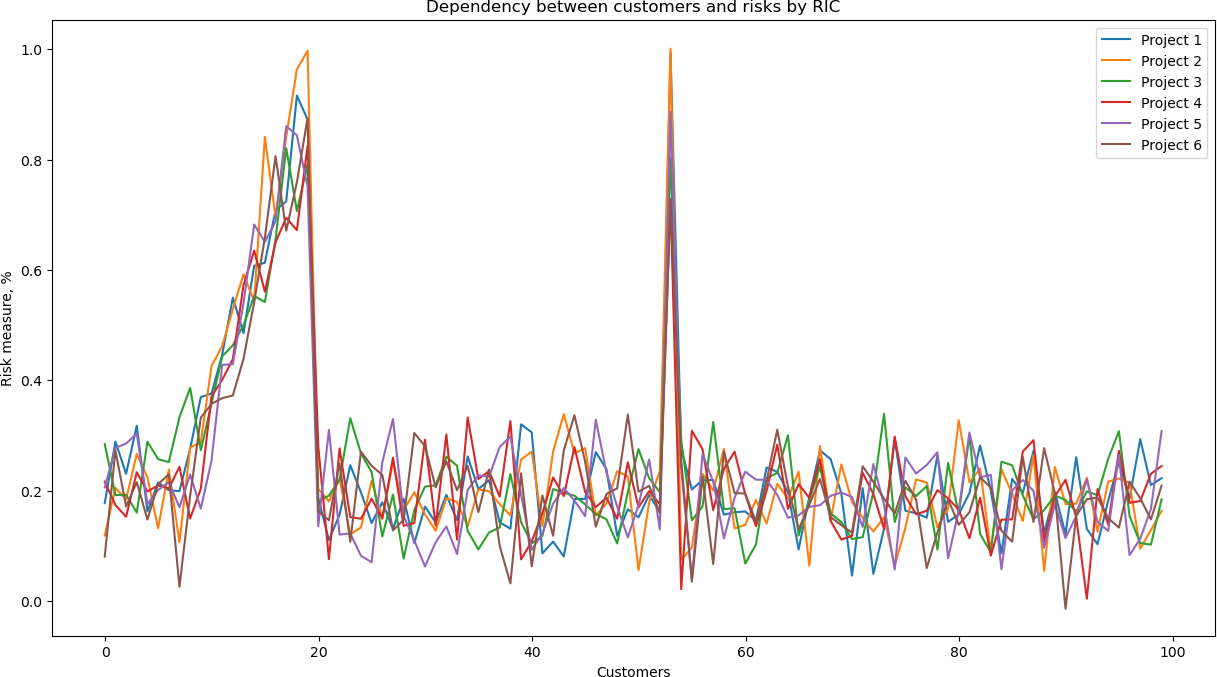
\includegraphics[width=0.8\textwidth]{media/ict2/image12}
	\caption*{Fig. 4 - Risk measurement by customers}
\end{figure}

\begin{multicols}{2}
The machine learning (ML) model further enhances the analysis by
leveraging these RIC metrics alongside other key data points to refine
investment predictions. The ML model integrates both time-series
analysis and sentiment analysis to capture trends and market sentiment,
offering a more comprehensive assessment of investment opportunities. By
utilizing algorithms and back testing procedures, the model incorporates
confidence levels and simulates real-world scenarios, effectively
identifying buying and selling points to optimize investment strategies.
The combination of RIC and ML-driven insights provides a robust
framework for evaluating investment risks.

The application of the RIC yielded varied results across the board,
reflecting a broad spectrum of investment reliability among the
companies analyzed. Notably, the formula demonstrated its utility in
distinguishing between high-risk and secure investment opportunities
based on quantifiable metrics. Several companies scored above 60\%,
indicating strong financial health and market position, thus making them
highly recommended for investment. Conversely, a few companies scored
below 30\%, suggesting significant risks that might outweigh potential
returns, as shown in Fig. 5.
\end{multicols}

\begin{figure}[H]
	\centering
	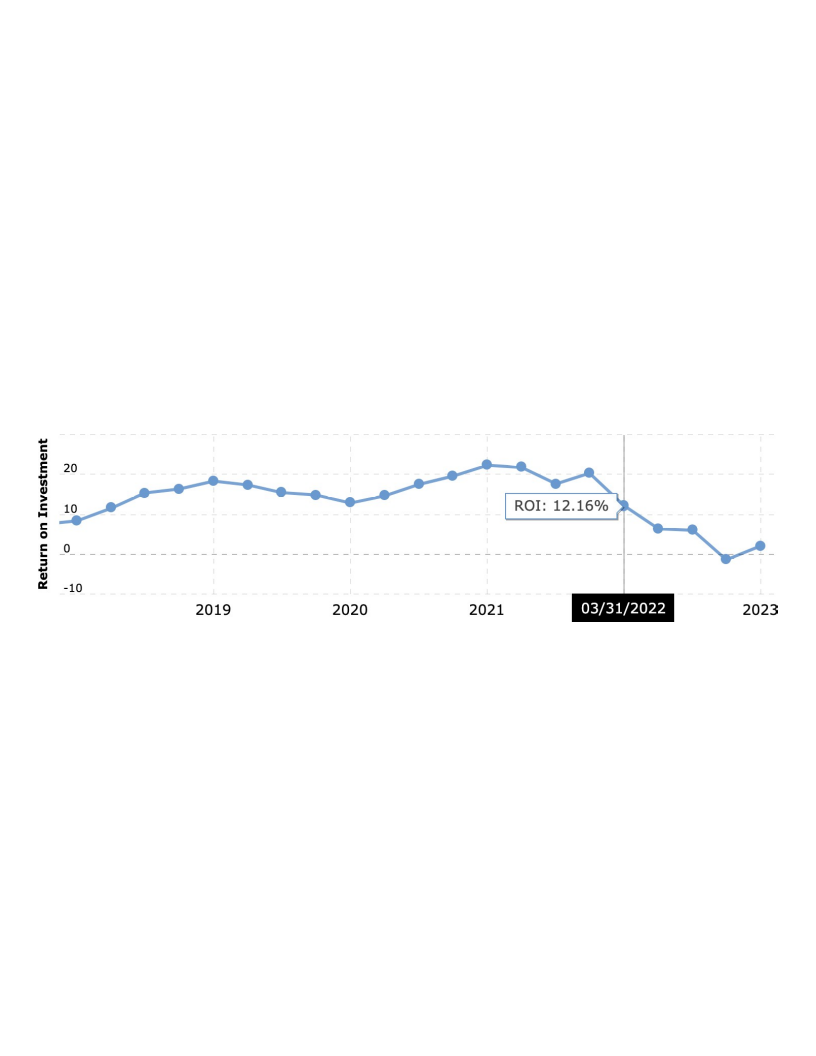
\includegraphics[width=0.8\textwidth]{media/ict2/image13}
	\caption*{Fig. 5 - ROI data for a 5-year period}
\end{figure}

\begin{multicols}{2}
The results from this empirical investigation confirm that the RIC
provides a robust framework for evaluating investment opportunities. By
quantifying risk and correlating it with market and financial data, the
formula helps investors make informed decisions grounded in
comprehensive analytics {[}14{]}. Moving forward, there are obvious
recommendations to refine the RIC parameters to enhance its predictive
accuracy and applicability across different economic cycles and industry
sectors. This ongoing validation process will ensure that the RIC
remains a reliable tool for investment assessment in the dynamic global
market (See Table 2). The machine learning model well complements the
RIC framework by incorporating advanced analytical techniques to refine
predictions and improve investment decisions. The model combines
time-series analysis and sentiment analysis to identify patterns and
gauge market sentiment, enriching the insights provided by the RIC.
\end{multicols}

\begin{table}[H]
\caption*{Table 2 - Investment assessment of the global market companies (NASDAQ)}
\centering
\begin{tblr}{
  cells = {c},
  hlines,
  vlines,
}
Company   & R (\%) & I (\%) & C (\%) & Result \\
Amazon    & 80     & 13.53  & 79     & 57.51  \\
Microsoft & 80     & 29.19  & 79     & 62.73  \\
AMD       & 60     & 19.89  & 78     & 52.63  \\
Intel     & 80     & 15.35  & 79     & 58.11  \\
Nokia     & 80     & 2.54   & 67     & 49.85  \\
IBM       & 80     & 9.13   & 68     & 52.37  \\
Netflix   & 80     & 12.48  & 79     & 57.16  \\
NVIDIA    & 70     & 24.73  & 85     & 59.91  \\
SAP       & 90     & 8.87   & 83     & 60.62  \\
Oracle    & 80     & 13.26  & 69     & 54.08  
\end{tblr}
\end{table}

\begin{multicols}{2}
The machine learning module collects data from various sources to train
predictive models. To preliminarily evaluate the usefulness of the data,
the employment of time-series analysis and sentiment analysis provides a
quick indication of whether valuable information is present. At this
stage, the module is dedicated solely to Buy/Sell prediction tasks. To
label the data, the authors devised a custom algorithm that greedily
assigns points into three categories by identifying buying and selling
points at the lowest and highest prices within a defined range. However,
this labeling approach introduces significant class imbalance, leading
the model to predominantly predict "hold," thereby failing to learn
meaningful patterns. The results of this approach are illustrated in
Fig. 6.
\end{multicols}

\begin{figure}[H]
	\centering
	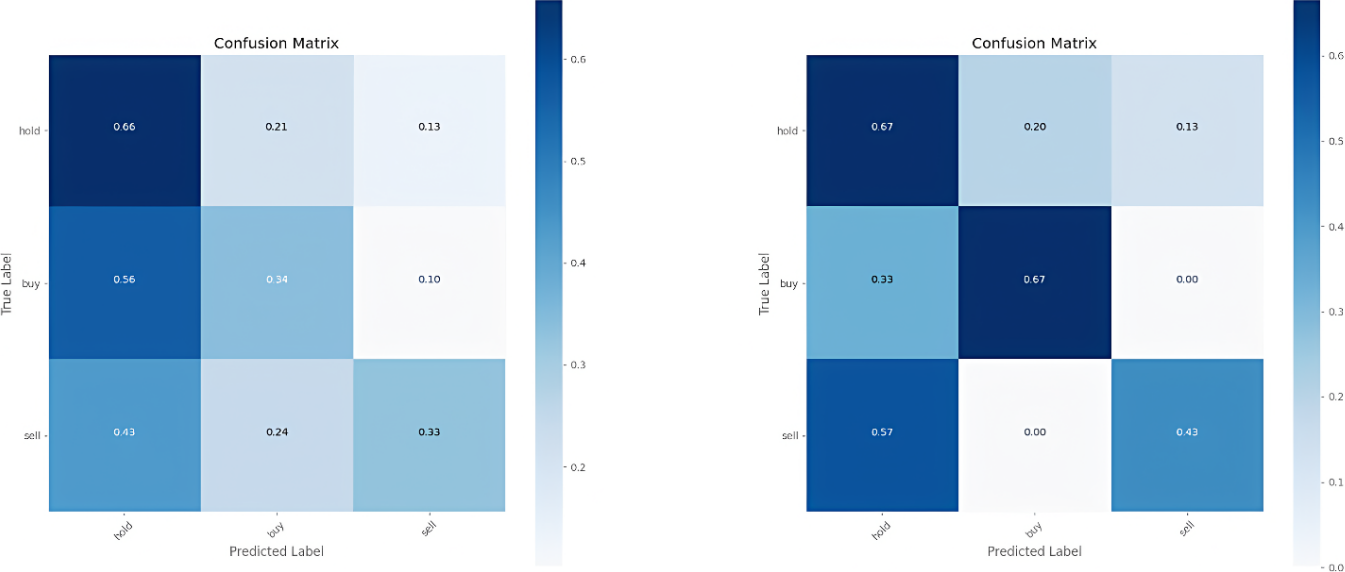
\includegraphics[width=0.8\textwidth]{media/ict2/image14}
	\caption*{Fig. 6 - Predicted investment decisions for the companies}
\end{figure}

\begin{multicols}{2}
Given the inherent difficulty of the task, there's been a question
whether the model could effectively identify upward and downward trends
necessary for accurate predictions, particularly as the confusion matrix
alone does not adequately capture its performance. To address this, the
study adopted a more practical evaluation metric by simulating
real-world conditions-investing funds and measuring potential returns.
It's been considered to implement a back testing strategy that
incorporates the model's confidence levels.

The application of the RIC across various companies and industries has
offered significant insights into the complexities of financial risk
assessment. Leveraging data from sources such as Macrotrends, Infront
Analytics, and Comparably, this study demonstrates the
formula' s ability to categorize companies into low,
medium, and high investment recommendation tiers based on their scores.
This stratification serves as a vital tool for investors aiming to make
data-driven decisions in a competitive market environment {[}15{]}.
Another key finding of this study is the RIC' s
reliability in delivering consistent risk assessments under diverse
economic conditions {[}16-17{]}. The formula' s
robustness lies in its capacity to integrate immediate financial metrics
with broader economic indicators, making it an adaptable framework even
in fluctuating markets.

One of the primary limitations of the RIC method lies in its reliance on
historical financial data and predefined risk thresholds, which may not
fully capture the dynamic processes of financial markets. The fixed risk
categories (30\%, 60\%) are based on past trends and economic theories,
making them potentially outdated in rapidly evolving conditions.
Additionally, while the RIC effectively quantifies investment risk using
financial indicators, it lacks the ability to incorporate qualitative
factors such as market innovation, or industry disruptions, elements
that can impact a company' s long-term performance. The
RIC method operates under the assumption that past performance is
indicative of future results, which may not always hold true in
speculative markets {[}18{]}. While the integration of machine learning
generally improves predictive capabilities, issues such as data
imbalance and overfitting can limit the accuracy of uncertain forecasts.

To address these limitations, this study introduces machine learning
(ML) techniques as a complementary approach to refine the framework. By
integrating ML models, such as time-series forecasting and sentiment
analysis, the RIC can incorporate a more dynamic and adaptive
methodology. For instance, the ML models analyze historical and
real-time market data to identify patterns, predict future trends, and
enhance the precision of RIC scores. Furthermore, advanced ML-driven
algorithms allow for the consideration of qualitative factors by
processing textual and sentiment data from news, reports, and social
media {[}19-20{]}. This holistic integration of quantitative and
qualitative metrics improves the RIC' s predictive
capabilities, enabling it to provide a more comprehensive assessment of
a company' s investment potential.

Future research should focus on optimizing the framework by
incorporating these ML advancements and exploring additional data
sources. By employing techniques such as neural networks, clustering,
and reinforcement learning, the RIC can evolve into a model that adapts
to market changes and investor behaviors in real time {[}21{]}. This
evolution will enhance the tool's utility for investors seeking
actionable insights in increasingly complex financial landscapes. The
RIC method provides a foundational yet flexible framework for assessing
and comparing the investment reliability of companies systematically.
While this study affirms its utility and relevance, the integration of
ML models and continuous validation with diverse datasets will be
essential for maintaining its effectiveness. As financial markets become
more interconnected and data-rich, the combination of the RIC framework
with advanced ML techniques will pave the way for a new generation of
investment assessment tools, capable of delivering better support.

{\bfseries Conclusion.} The application of the RIC method in this study has
demonstrated its efficacy in evaluating investment opportunities with
above 80\% risk score. By incorporating both tangible and intangible
factors, the formula provides a comprehensive tool for assessing the
attractiveness of investments. This practical approach is crucial for
capturing the full spectrum of influences that can impact investment
decisions. The findings indicate that the method enables quick and
accurate determination of investment viability, supporting its use as a
reliable decision-making tool in financial analysis. The success of this
initial application suggests that the formula performs well across a
diverse range of company types and sizes, from emerging businesses to
large global corporations in the IT sector.

Given the positive results, future research is planned to refine and
potentially expand the criteria used in the RIC method. Considerations
such as Cost Benefit Analysis and Return on Assets could be integrated
to enhance the formula' s accuracy and relevance. Such
developments could lead to a more precise method for assessing
investments, tailored to the specific needs and contexts of various
companies, thereby supporting investors in making even more informed
decisions. The continual improvement and testing of the method will be
essential to adapt to the evolving economic landscapes and investment
scenarios, ensuring that it remains a robust tool in the arsenal of
financial analysts and investors worldwide.
\end{multicols}

\begin{center}
{\bfseries References}
\end{center}

\begin{references}
1. Ilin V., Levina A., Dubgorn A., Abran A. Investment Models for
Enterprise Architecture and IT \\Architecture Projects within the Open
Innovation Concept // Journal of Open Innovation: Tech, Market, and
Complex. -2021. -Vol. 7. -P. 1-18. DOI
\href{https://doi.org/10.3390/joitmc7010069}{10.3390/joitmc7010069}.

2. Purwita W., Subriadi A. P. Information Technology Investment: In
Search of the Closest Accurate Method // Procedia Computer Science.
-2019.-Vol.161.-P.300 -307.
DOI \href{https://doi.org/10.1016/j.procs.2019.11.127}{10.1016/j.procs.2019.11.127}.

3. Meyer R., Degoulet P. Choosing the Right Amount of Healthcare
Information Technologies Investments // International Journal of Medical
Informatics.-2010.- Vol. 79.-P. 225--231. DOI:\\
\href{https://doi.org/10.1016/j.ijmedinf.2010.01.001}{10.1016/j.ijmedinf.2010.01.001}.

4. Ali S., Green P., Robb A. Information Technology Investment
Governance: What Is It and Does It Matter? // International Journal of
Accounting Information Systems. -2015. -Vol.18. -P.1-25. DOI\\
\href{https://doi.org/10.1016/j.accinf.2015.04.002}{10.1016/j.accinf.2015.04.002}.

5. Berghout E., Tan C. W. Understanding the Impact of Business Cases on
IT Investment Decisions: An Analysis of Municipal E-Government Projects
// Information and Management. - 2013.- Vol.50. - P. 489-506. - DOI
\href{https://doi.org/10.1016/j.im.2013.07.010}{10.1016/j.im.2013.07.010}.

6. Chen P. S., Yen D. C., Lin S. C., Chou C. S. Toward an IT Investment
Decision Support Model for Global Enterprises//Computer Standards and
Interfaces. -2018.-Vol. 59. -P.130-140.
DOI \\\href{http://dx.doi.org/10.1016/j.csi.2018.04.001}{10.1016/j.csi.2018.04.001}.

7. Witra W. P. P., Subriadi A. P. Gender and Information Technology (IT)
Investment Decision-Making // Procedia Computer Science.-2021.-Vol.197.-P.
583-590.-
DOI \href{https://doi.org/10.1016/j.procs.2021.12.176}{10.1016/j.procs.2021.12.176}.

8. Mirza S. S., Majeed M. A., Ahsan T. Board Gender Diversity,
Competitive Pressure and Investment Efficiency in Chinese Private Firms
// Eurasian Business Review.-2020.-Vol.10(3).- P. 417-440. DOI:
\href{https://doi.org/10.1007/s40821-019-00138-5}{10.1007/s40821-019-00138-5}.

9. Shin Y. Z., Chang J. Y., Jeon K. et al. Female Directors on the Board
and Investment Efficiency: Evidence from Korea // Asian Business \&
Management.- 2020.-Vol.19.-P. 438-479.
DOI \href{https://doi.org/10.1057/s41291-019-00066-2}{10.1057/s41291-019-00066-2}.

10. Lee H., Choi H., Lee J., Min J., Lee H. Impact of IT Investment on
Firm Performance Based on Technology IT Architecture // Telematics and
Informatics.-2016.-Vol.91. -P. 652-661.
DOI \\\href{https://doi.org/10.1016/j.procs.2016.07.164}{10.1016/j.procs.2016.07.164}.

11. Macrotrends -Website with Financial Data. URL:
https://www.macrotrends.net.Accessed: 18.02.2025.

12. Infront Analytics -Website with Financial Data. URL:
https://infrontanalytics.com. Accessed: \\18.02.2025.

13. Comparably-Website with Financial
Data.URL:https://www.comparably.com/brands/ Accessed: \\18.02.2025.

14. Suchkov M., Bekturgan B., Kartbayev A. Gamification Effects on
Employee Engagement and Business Process Risk Evaluation // 2024 IEEE
4th International Conference on Smart Information Systems and
Technologies (SIST).-Astana, Kazakhstan, 2024.- P. 594--599.
DOI \href{https://doi.org/10.1109/SIST61555.2024.10629629}{10.1109/SIST61555.2024.10629629}.

15. Gao Y., Zhao C., Sun B., Zhao W. Effects of Investor on Stock
Volatility: New Evidences from Multi-Source Data in
China' s Green Stock Markets // Financial
Innovation.-2022.- Vol. 8(1).- Art. 77. - P. 1-30. DOI
\href{https://doi.org/10.1186/s40854-022-00381-2}{10.1186/s40854-022-00381-2}

16. Zhang F., Ding Y., Liao Y. Financial Data Collection Based on Big
Data Intelligent Processing // International Journal of Information
Technology and Systems Approach. -2023.- Vol.16( 3). - P. 1--13. DOI
10.4018/IJITSA.320514.

17. Sonkavde G., Dharrao D. S., Bongale A. M., Deokate S. T., Doreswamy
D., Bhat S. K. Forecasting Stock Market Prices Using Machine Learning
and Deep Learning Models: A Systematic Review, \\Performance Analysis, and
Discussion of Implications // International Journal of Financial
Studies.-2023.-Vol. 11. - Art. 94. DOI
\href{https://doi.org/10.3390/ijfs11030094}{10.3390/ijfs11030094}.

18. Bhowmik R., Wang S. Stock Market Volatility and Return Analysis: A
Systematic Literature Review // Entropy. -2020. - Vol. 22(5). -Art. 522.
DOI \href{https://doi.org/10.3390/e22050522}{10.3390/e22050522}.

19. Gong X., Wang C., Zhang W., Wang J. Investor Sentiment and Stock
Volatility: New Evidence // International Review of Financial
Analysis.-2022.-Vol.81.-Art.102008.
DOI:\href{http://dx.doi.org/10.1016/j.irfa.2022.102028}{10.1016/j.irfa.2022.102028}.

20. Rouatbi W., Demir E., Kizys R., Zaremba A. Immunizing Markets Against
the Pandemic: COVID-19 Vaccinations and Stock Volatility Around the
World // International Review of Financial Analysis. - 2021.-Vol.76.-
Art. 101785. DOI \href{https://doi.org/10.1016/j.irfa.2021.101819}{10.1016/j.irfa.2021.101819}.

21. Chevallier J., Ma F., Guo Y., Huang D. Macroeconomic Attention,
Economic Policy Uncertainty, and Stock Volatility Predictability //
International Review of Financial Analysis. - 2022. -Vol.81. -Art.
102037. DOI \href{https://doi.org/10.1016/j.irfa.2022.102339}{10.1016/j.irfa.2022.102339}.
\end{references}

\begin{authorinfo}
\emph{{\bfseries Information about the authors}}

Bolatova A.- master student, Kazakh-British Technical University,
Almaty, Kazakhstan, aru\_bolatova@kbtu.kz;

Kylyshbek U.- master student, Kazakh-British Technical University,
Almaty, Kazakhstan, u\_kylyshbek@kbtu.kz;

Baktygaliyev A.- master student, Kazakh-British Technical University,
Almaty, Kazakhstan, a\_baktygaliyev@kbtu.kz;

Kartbayev A.- PhD, associate professor, Kazakh-British Technical
University, Almaty, Kazakhstan, a.kartbaev@kbtu.kz

\emph{{\bfseries Сведения об авторах}}

Болатова А.- магистрант, Казахстанско-Британский технический
университет, Алматы, Казахстан, \\aru\_bolatova@kbtu.kz;

Кылышбек У.- магистрант, Казахстанско-Британский технический
университет, Алматы, Казахстан, \\u\_kylyshbek@kbtu.kz;

Бактыгалиев А.- магистрант, Казахстанско-Британский технический
университет,

Алматы, Казахстан, a\_baktygaliyev@kbtu.kz;

Картбаев А. PhD, ассоциированный профессор, Казахстанско-Британский
технический университет, Алматы, Казахстан, a.kartbaev@kbtu.kz
\end{authorinfo}
